\section{Data Sources}
\label{app:data-sources}
This appendix gives per-source descriptions of the input modalities summarized in \S\ref{ssec:arch-inputs}, organized by the risk component each contributes to.

\subsection{Hazard: Hydrometeorology}
\paragraph{NOAA Analysis of Record for Calibration (AORC)}
High quality record of precipitation with sufficient temporal and spatial resolution is critical to account for flood damages.
%
Past works have employed a variety of precipitation records including NASA's IMERG~\cite{huffman_integrated_2020} or ERA5~\cite{hersbach_era5_2020} reanalysis data; however, these datasets are insufficient for the daily, $\sim$1km scale of our analysis.
%
In this work, we use the NOAA Analysis of Record for Calibration (AORC) dataset~\cite{fall_analysis_2023}, which provides a high quality, high resolution (hourly, $\sim$800m) precipitation record for the Conterminous United States.
%
We use the \textbf{\textit{Hourly Accumulated Precipitation}} record from this archive.

\paragraph{NOAA National Water Model (NWM) Retrospective}
Precipitation signal alone is often insufficient to model pluvial flood occurrence and intensity, as past works have shown that pluvial flooding is fundamentally a hydrological problem~\cite{james_precipitation_2024}.
%
Thus to supplement the NOAA AORC precipitation records, we turn to NOAA's National Water Model (NWM) Retrospective dataset v3.0~\cite{cosgrove_noaas_2024} available from Feb. 1979 to Jan. 2023.
%
Amongst its various outputs, we use the Land Surface Model component, which provides 3-hourly records of physical land surface and hydrologic states at $\sim$1\,km resolution.
%
We use two variables from the NWM Retrospective dataset: \textbf{\textit{Volumetric Soil Moisture}} and \textbf{\textit{Snow Water Equivalent}}.

\subsection{Hazard: Terrain}

\paragraph{Topographic Wetness Index (TWI)}
\textbf{\textit{Topographic Wetness Index}} quantifies the steady-state propensity of a location to accumulate surface water from its upslope contributing area, defined as $\mathrm{TWI} = \ln(a/\tan\beta)$, where $a$ is the upslope contributing area per unit contour length and $\beta$ is the local slope.
%
We use the CONUS-wide 30m product from~\cite{hoylman_30m_2021}.

\paragraph{Height Above Nearest Drainage (HAND)}
\textbf{\textit{Height Above Nearest Drainage}} measures the vertical elevation of each cell above its hydrologically connected drainage network.
%
Low-HAND cells lie nearest the drainage corridors that inundate first when local drainage capacity is exceeded, making HAND a direct proxy for pluvial flood susceptibility.
%
We use the Copernicus DEM HAND dataset at 30\,m resolution~\cite{aws_copernicus_dem}.

\paragraph{Global Curve Number (GCN)}
The SCS Curve Number parameterizes surface runoff potential as a joint function of soil hydrologic group and land cover, with values ranging from $\sim$30 (high infiltration on sandy or forested terrain) to 100 (fully impervious surfaces).
%
Higher CN indicates a larger fraction of incident precipitation converted to surface runoff, the proximate hydrologic driver of pluvial flooding.
%
CN values from~\cite{jaafar_gcn250_2019} are derived from three different antecedent runoff conditions (ARC): dry (ARC I), average (ARC II), and wet (ARC III) soil moisture states, which we include as separate features.
%
We use the three \textbf{\textit{Global Curve Numbers}} as terrain hazard descriptors.

\paragraph{NLCD Land Cover}
Land cover plays an important role in pluvial flood risk with impervious surfaces generating more runoff and thus more pluvial flood risk.
%
To account for impervious surfaces, we include the National Land Cover Database (NLCD) 2016 product~\cite{usgs_annual_nlcd_2024}, which provides 30m land cover classifications across the Conterminous United States.
%
We use the \textbf{\textit{Fractional Impervious Surface}} classification as a surface descriptor.

\paragraph{POLARIS Soil Properties}
Soil plays a critical role in modeling pluvial flood events~\cite{rong_impact_2024}, as it controls the partitioning of precipitation into infiltration and runoff.
%
To account for the varied soil properties across the Conterminous United States, we include the POLARIS dataset~\cite{chaney_polaris_2019}, which provides high-resolution (30m) estimates of soil properties such as texture, hydraulic conductivity, and water retention characteristics.
%
From the dataset, we identify three variables of interest: $K_{sat}$, the \textbf{saturated hydraulic conductivity} (\emph{$\log_{10}(cm/hr)$}); \emph{clay}, the \textbf{clay percentage} (\%); and $\theta_{s}$, the \textbf{saturated soil water content} ($m^3/m^3$).
%
All values are derived from the 0--5\,cm soil layer.

\subsection{Exposure and Vulnerability}
\paragraph{FIMA NFIP Policies}
The FIMA NFIP policies dataset provides spatially aggregated counts and total coverage of active flood insurance policies across the Conterminous United States.
%
We use policy density and total insured value as exposure proxies; regions with denser NFIP coverage contain more structures with known flood vulnerability and a larger insured asset base at risk.
%
These are derived from the OpenFEMA FIMA Redacted Policies Dataset v2~\cite{fema_nfip_policies_v2} and undergo the same spatial uncertainty correction as the claims data (\S\ref{ssec:spatial_correction}), yielding a polygon-level count and total coverage for each cell in our analysis grid.
%
We derive \textbf{\textit{\# Active NFIP Policy}} from this archive.

\paragraph{National Structure Inventory (NSI)}
The U.S. Army Corps of Engineers National Structure Inventory~\cite{usace_nsi_2022} provides a point-level inventory of structures across CONUS, with per-structure attributes including replacement value, occupancy type, square footage, first-floor elevation, and foundation type.
%
From this archive we derive and rasterize using the same methodology as in \S\ref{ssec:spatial_correction} the following variables: \textbf{Total Count of Structures}, \textbf{\% Structs with Basements}, \textbf{\% Struct. with Slab Foundation}, \textbf{\% Mobile Homes}, \textbf{\% Structs in Special Flood Hazard Area (SFHA)}, and \textbf{Average, Min, Standard Deviation First Floor Elevation}.

\subsection{Google AlphaEarth Foundation (AEF)}
The AlphaEarth Foundation model provides a 64-dimensional learned embedding of Earth's surface at 10\,m resolution, trained on multi-source Earth observation imagery and other environmental datasets~\cite{brown_alphaearth_2025}.
%
AEF embeddings implicitly encode land cover, impervious surface fraction, urbanization patterns, vegetation, and built-environment morphology, all factors that modulate runoff generation and drainage capacity, providing a complementary, dense representation alongside the hand-engineered terrain and exposure features above.

\subsection{Normalization}
To stabilize training, we apply transformations to our raw feature values.
%
For those that exhibit high right skew, \textbf{HAND}, \textbf{TWI}, \textbf{\# Active NFIP Policies}, \textbf{\# NSI Structures}, we apply a $\ln(x+1)$ transformation followed by a z-score normalization.
%
For \textbf{NSI Foundation height features}, we apply a z-score normalization without the log transform, as these features are not as heavily skewed.
%
For the rest we apply a min-max normalization to scale values to the [0,1] range.
\section{Date Shift Distribution}
We describe our temporal correction procedure in \S\ref{ssec:temporal_correction}. 
%
Here, we report the distribution of date shifts $\Delta = d' - d$ applied to the original NFIP claim dates $d$ to obtain the corrected dates $d'$ used in our study region. As shown in Table~\ref{tab:date_shifts}, the vast majority of claims ($81.1\%$) had no date shift, while $7\%$ has shifts of $\pm 1$ day and $6\%$ were discarded.
\begin{table}[h]
\small
\centering
\setlength{\tabcolsep}{5pt}
\begin{tabular}{r *{8}{c}}
\toprule
$\Delta$ (days) & $-3$ & $-2$ & $-1$ & $\phantom{-}0$ & $+1$ & $+2$ & $+3$ & -- \\
\midrule
\% & $2.0$ & $1.9$ & $5.0$ & $\mathbf{81.1}$ & $2.0$ & $1.4$ & $0.6$ & $6.0$ \\
\bottomrule
\end{tabular}
\caption{Distribution of date shifts $\Delta = d' - d$ from the temporal correction. (See \S\ref{ssec:study_region})}
\label{tab:date_shifts}
\end{table}

\section{All Held-Out Cell Modulator Dynamics}
\label{app:all-cell-dynamics}
For completeness, Figures~\ref{fig:all-cell-basemaps},~\ref{fig:all-aef-cluster} and~\ref{fig:all-cell-kernels} show, respectively, the basemap, the AEF clustering, and the learned modulator clustering for every held-out cell. Panel positions match across the three figures.

\begin{figure*}[!ht]
\centering
\setlength{\tabcolsep}{1pt}
\renewcommand{\arraystretch}{0.4}
\newcommand{\cellbasemap}[1]{\includegraphics[width=0.15\textwidth]{figs/cell_dynamics_val_cell_#1_basemap.pdf}}
\begin{tabular}{cccccc}
\cellbasemap{60}   & \cellbasemap{1132} & \cellbasemap{1136} & \cellbasemap{1179} & \cellbasemap{1330} & \cellbasemap{1331} \\
\cellbasemap{1412} & \cellbasemap{1486} & \cellbasemap{1487} & \cellbasemap{1490} & \cellbasemap{1526} & \cellbasemap{1544} \\
\cellbasemap{1605} & \cellbasemap{1644} & \cellbasemap{1648} & \cellbasemap{1658} & \cellbasemap{1683} & \cellbasemap{1779} \\
\cellbasemap{1874} & \cellbasemap{1914} & \cellbasemap{1917} & \cellbasemap{1933} & \cellbasemap{1999} & \cellbasemap{2091} \\
\cellbasemap{2166} & \cellbasemap{2168} & \cellbasemap{2170} & \cellbasemap{2208} & \cellbasemap{2209} & \cellbasemap{2288} \\
\end{tabular}
\caption{Basemaps of all 30 held-out cells, paired with the modulator kernels in Figure~\ref{fig:all-cell-kernels}}
\label{fig:all-cell-basemaps}
\end{figure*}
\begin{figure*}[!ht]
\centering
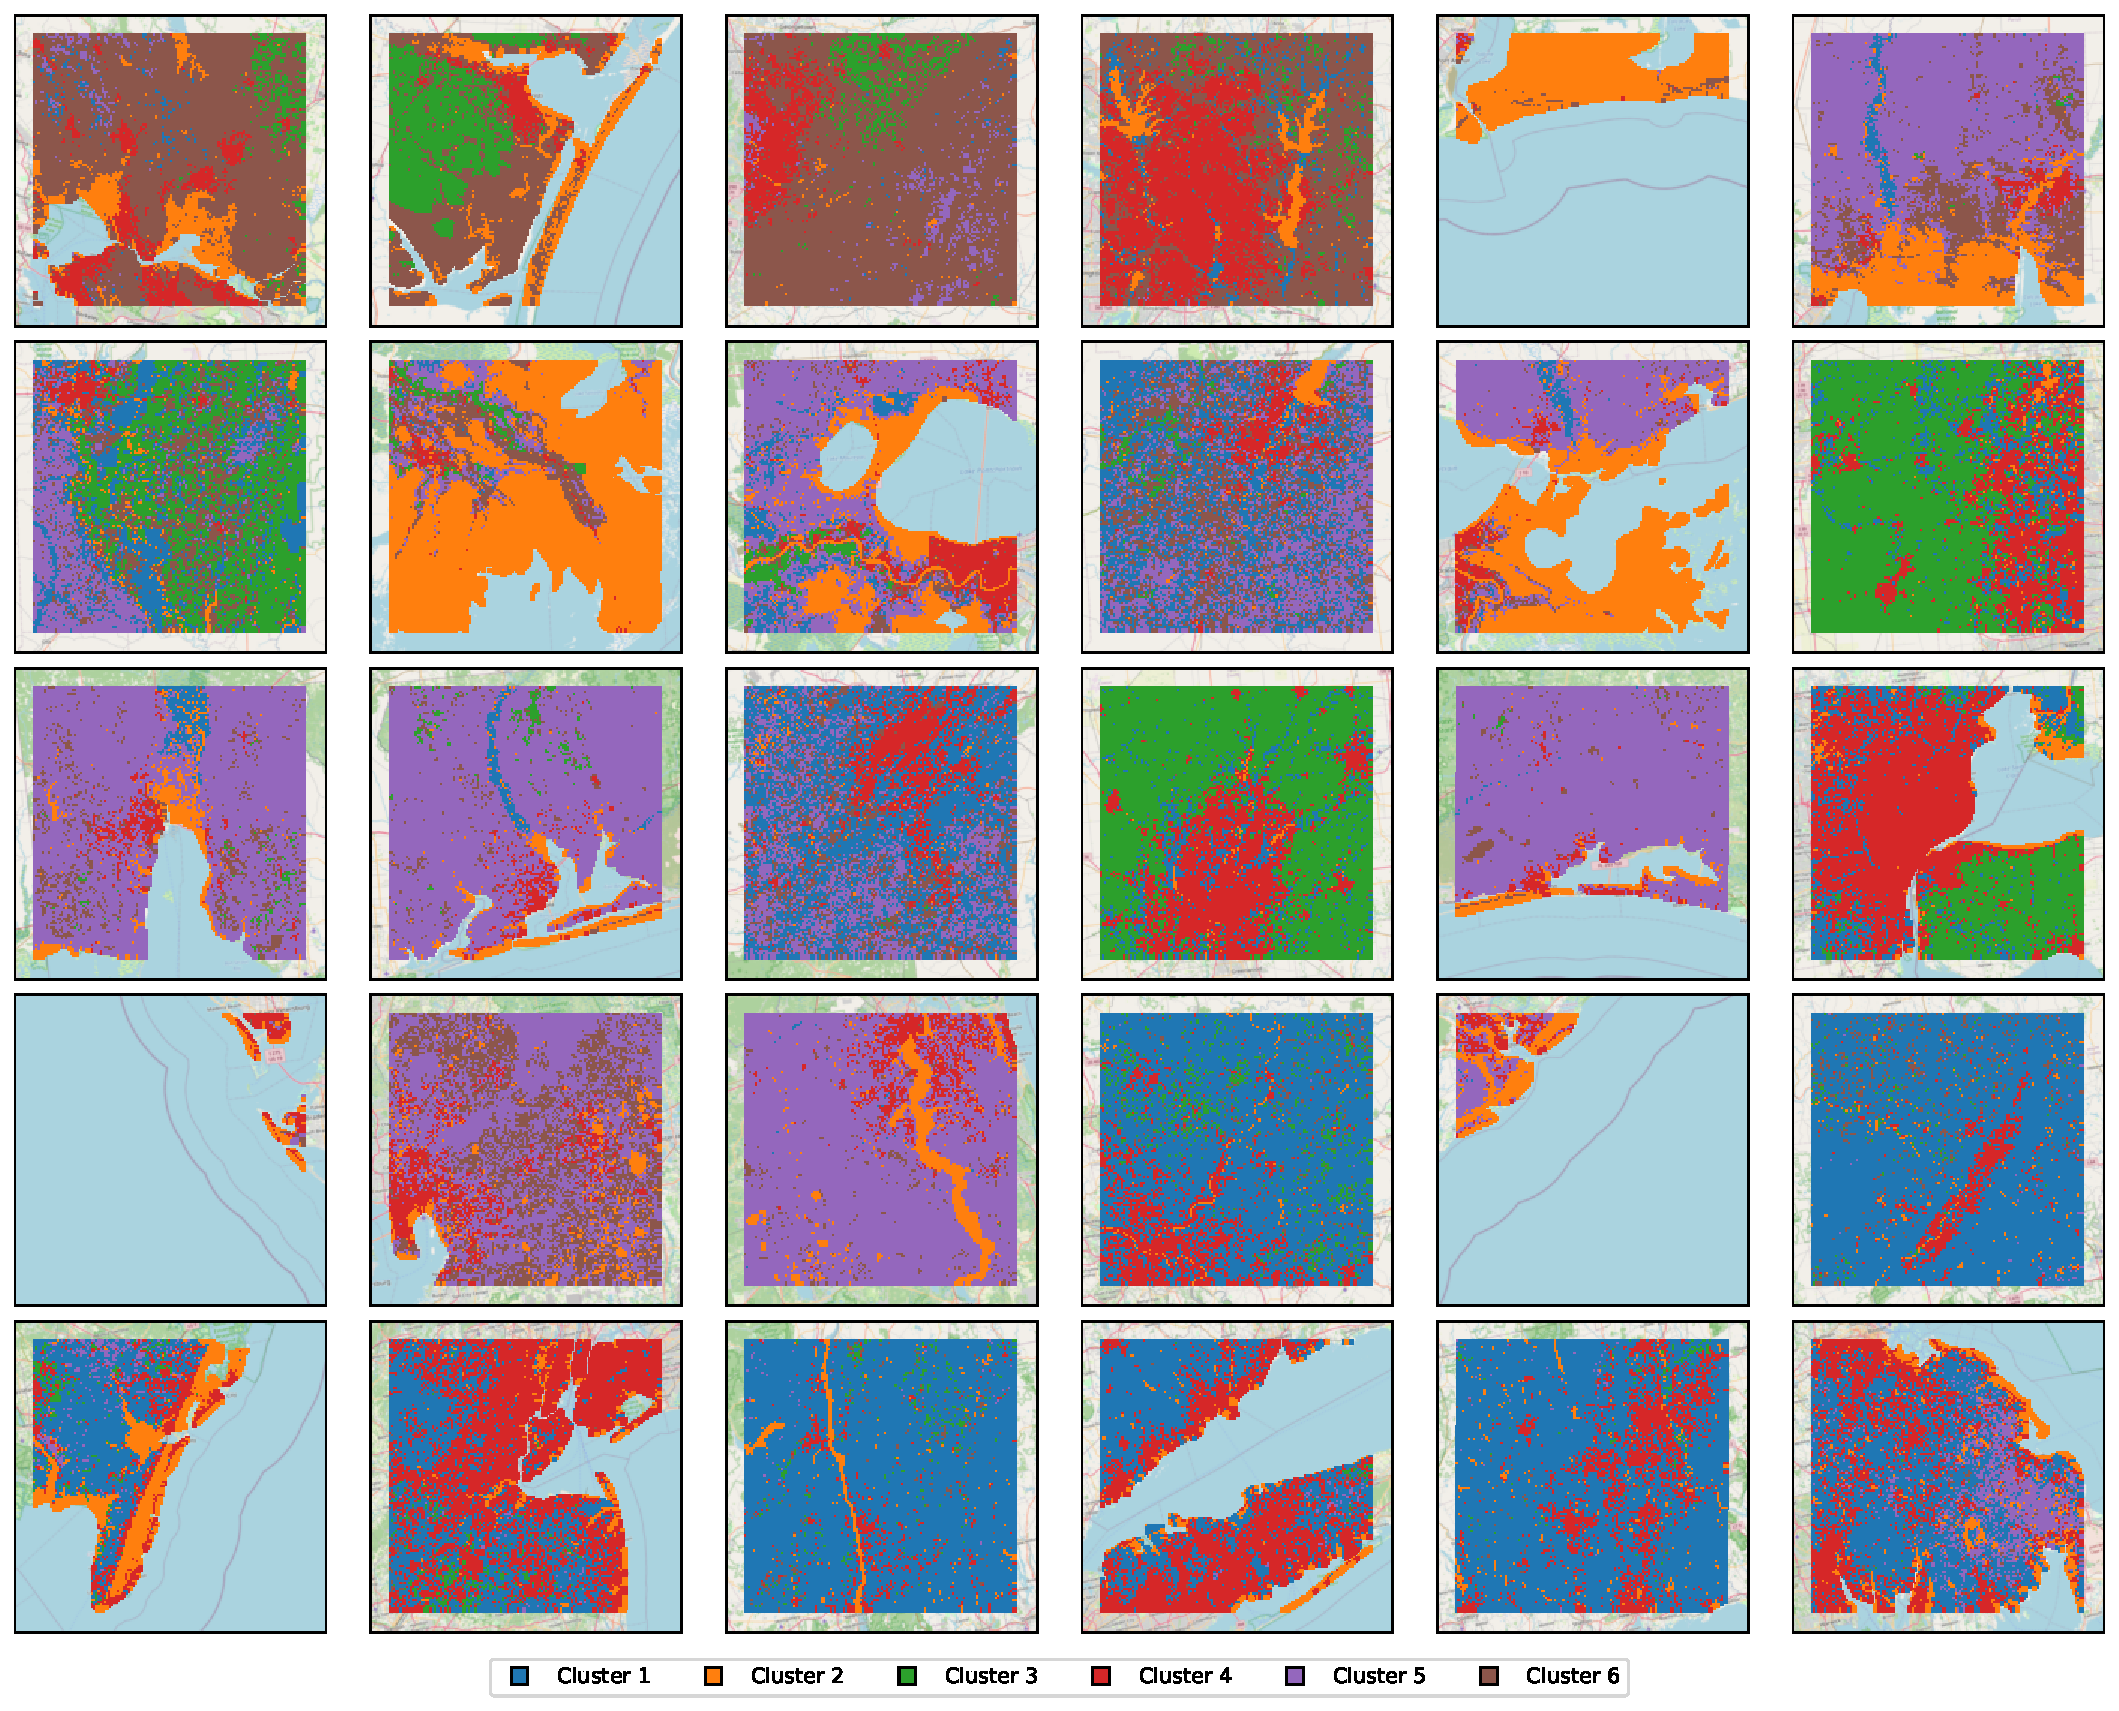
\includegraphics[width=\textwidth]{figs/aef_cluster_per_cell.pdf}
\caption{Google AlphaEarth Clustering results for all 30 held-out cells. See \S\ref{ssec:loc_char}.}
\label{fig:all-aef-cluster}
\end{figure*}

\begin{figure*}[!ht]
\centering
\setlength{\tabcolsep}{1pt}
\renewcommand{\arraystretch}{0.4}
\newcommand{\cellkernel}[1]{\includegraphics[width=0.15\textwidth]{figs/cell_dynamics_val_cell_#1.pdf}}
\begin{tabular}{cccccc}
\cellkernel{60}   & \cellkernel{1132} & \cellkernel{1136} & \cellkernel{1179} & \cellkernel{1330} & \cellkernel{1331} \\
\cellkernel{1412} & \cellkernel{1486} & \cellkernel{1487} & \cellkernel{1490} & \cellkernel{1526} & \cellkernel{1544} \\
\cellkernel{1605} & \cellkernel{1644} & \cellkernel{1648} & \cellkernel{1658} & \cellkernel{1683} & \cellkernel{1779} \\
\cellkernel{1874} & \cellkernel{1914} & \cellkernel{1917} & \cellkernel{1933} & \cellkernel{1999} & \cellkernel{2091} \\
\cellkernel{2166} & \cellkernel{2168} & \cellkernel{2170} & \cellkernel{2208} & \cellkernel{2209} & \cellkernel{2288} \\
\end{tabular}
\caption{Learned modulator clustering for all 30 held-out cells. See \S\ref{ssec:modulator_behaviors}. }
\label{fig:all-cell-kernels}
\end{figure*}


\section{Temporal Generalization}
Under a strict temporal split (train 2017--2020, test 2021--2022, single split), DELUGE retains its lead on both PR-AUC and \$-Weighted PR-AUC (Table~\ref{tab:temporal}).
%
PR-AUC degrades only modestly from the spatial split, with DELUGE the least affected at a \tsim$3\%$ drop and the tree baselines down \tsim$7$ to $10\%$, preserving DELUGE's lead and the baseline ordering.
%
\$-Weighted PR-AUC drops sharply for every model (roughly \tsim$38$ to $41\%$ from the spatial split), but DELUGE retains its lead and the ordering across baselines is preserved.
%
\begin{table}[h]
\small
\centering
\setlength{\tabcolsep}{4pt}
\begin{tabular}{l r r r r}
\toprule
\textbf{Model} & \textbf{PR-AUC} & \textbf{$\Delta$} & \textbf{\$-W PR-AUC} & \textbf{$\Delta$} \\
\midrule
\textbf{DELUGE (Ours)} & $\mathbf{0.237}$ & --      & $\mathbf{0.370}$ & --      \\
XGBoost                & $0.197$          & $-$17\% & $0.303$          & $-$18\% \\
LightGBM               & $0.212$          & $-$11\% & $0.329$          & $-$11\% \\
\bottomrule
\end{tabular}
\caption{\textbf{Temporal split (train 2017--2020, test 2021--2022, single split).} DELUGE retains its lead on both metrics.}
\label{tab:temporal}
\end{table}
%
The divergence between metrics is structural. 
%
PR-AUC averages over all positives whereas \$-Weighted PR-AUC concentrates on the few costliest claims, so models are judged primarily on how well they rank the tail.
% %
% And the tails of the two windows differ in obviousness. 
%
Training is dominated by Hurricane Harvey in 2017 (\$5.8B, more than the other three training years combined at \$2.0B), a clear signal that any reasonable model can learn to flag. 
%
Test years (\$1.4B in 2021, \$1.9B in 2022) lack a comparably obvious extreme, which hampers the \$-Weighted PR-AUC of all models.

\section{Performance Comparison by Location Characteristics}\label{ssec:loc_char}
To understand whether DELUGE's headline performance is uniform across our study cells or concentrated in particular locations, we stratify the held-out cells by their underlying landscape and report PR-AUC within each stratum.
%
We characterize each held-out pixel by its AlphaEarth Foundation embedding~\cite{brown_alphaearth_2025} and cluster the resulting per-pixel vectors with K-means and a silhouette sweep selects $K=6$.
%
We then report DELUGE's PR-AUC within each AEF cluster (Table~\ref{tab:loc-char}), along with the \emph{lift over prevalence} (PR-AUC $/$ prevalence), the multiplicative gain over a random predictor.
%
Inspecting the clusters' geographic membership, we label them as seen in Table~\ref{tab:loc-char}.
% : \textbf{C1} Northeast developed areas, \textbf{C2} coastal wetland, \textbf{C3} inland developed areas, \textbf{C4} dense developed areas, \textbf{C5} Southeast mixed rural-developed, and \textbf{C6} inland less-developed areas.
%
DELUGE's raw PR-AUC varies substantially across these strata.
%
Lift over prevalence largely controls for this, and across most clusters the gain over chance is comparable.

Of note, however, is the poor relative lift of the \textbf{dense developed} cluster (C4, $42\times$).
%
Despite the highest raw PR-AUC of any built-environment stratum, DELUGE's marginal contribution over a base-rate predictor is the smallest here.
%
We attribute this to \textbf{local, sub-kilometer flood dynamics in dense urban areas, that operate below the ${\sim}1$\,km resolution at which DELUGE operates.}
%
This matches the localization failure mode to be discussed in \S\ref{ssec:failure-modes} and points to spatial resolution as a natural lever for future work in this regime.
%
We place the full cluster membership and geographic distribution in Appendix.

\begin{table}[t]
\small
\centering
\setlength{\tabcolsep}{4pt}
\begin{tabular}{l r r r}
\toprule
\textbf{Cluster}  & \textbf{Prev. (\%)} & \textbf{PR-AUC} & \textbf{Lift} \\
\midrule
C1: NE developed             & $0.139$ & $0.184$         & $132{\times}$ \\
C2: Coastal wetland          & $0.166$ & $0.138$         & $83{\times}$ \\
C3: Inland developed         & $0.065$ & $0.080$         & $124{\times}$ \\
C4: Dense developed          & $0.610$ & $0.255$         & $42{\times}$ \\
C5: SE mixed rural-developed & $0.249$ & $0.322$ & $129{\times}$ \\
C6: Inland less-developed    & $0.222$ & $0.238$         & $107{\times}$ \\
\bottomrule
\end{tabular}
\caption{DELUGE performance stratified by AEF cluster. Held-out cells grouped by K-means ($K=6$) on the center-pixel AlphaEarth embedding. Prev.\ is per-pixel-day prevalence and lift is PR-AUC $/$ prevalence, the multiplicative gain over a random predictor.}
\label{tab:loc-char}
\end{table}

